\section{Model}

\subsection{Architecture Selection}

Deep Neural Networks (DNNs) are systems that learn to perform tasks from examples without prior knowledge of the task. Their capacity is controlled by varying their layers' depth and breadth, and they make assumptions that are strong and mostly correct \cite{krizhevsky2012alexnet}. Compared to traditional feed-forward neural networks, Convolutional Neural Networks (CNNs) have much fewer connections/parameters while retaining a similar upper bound in performance as DNNs. CNNs operate by employing layers of feature maps that filter for representative pixel intensities found through stochastic gradient descent (SGD) (Figure \ref{fig:BayesCNNwithdist}). Feature signals are then boosted through transformations \cite{Oquab2014} such as filtering and pooling which involve convolutional and statistical (i.e. average, max, norm, etc.) operations respectively. This interleaving of convolutions, pooling, and dense layers constructs a feature hierarchy that is invariant to image translation and exponentially more computationally efficient. 

In practice, traditional neural network architectures are over-confident predictors. This is because the expressiveness of CNNs makes them overfit smaller datasets, thereby performing well during training but poorly during testing. Various regularization techniques \cite{dialameh2020dlreg} exist for preventing overfitting (i.e. early stopping, weight decay, dropout, etc.). However, using single-point estimates for real world decisions is unjustifiable. Thus, by introducing Bayesian learning to the weights and final prediction of the network (Figure \ref{fig:BayesCNNwithdist}) we both counter overfitting and add a measure of uncertainty and regularization at inference time. \cite{shridhar2019comprehensive}.

\begin{figure}[!htb]
  \centering
  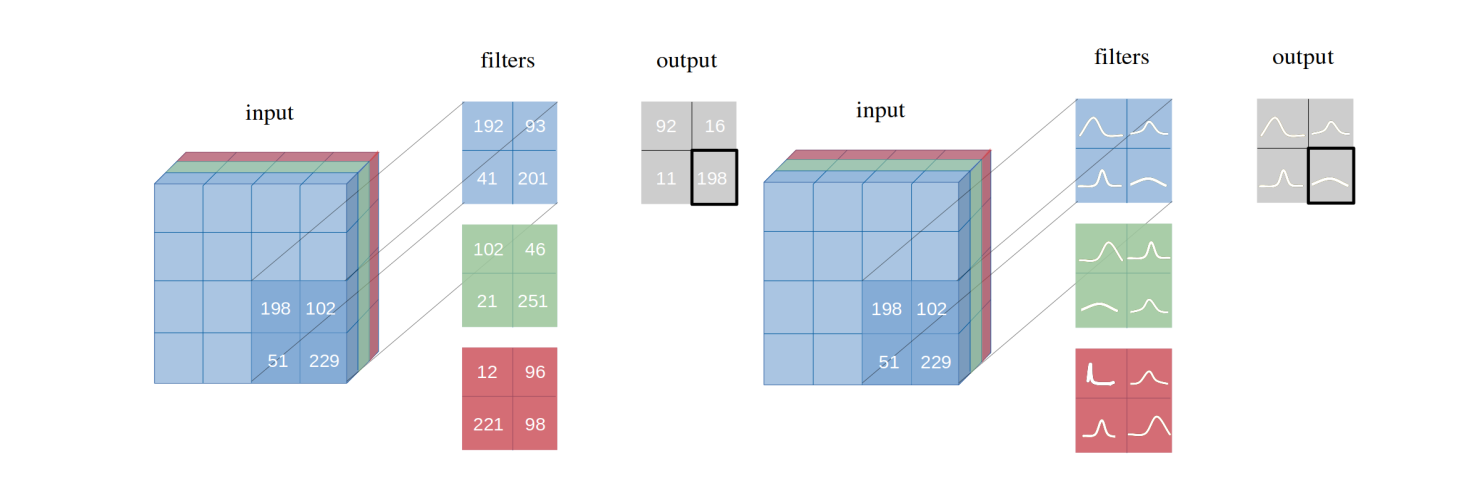
\includegraphics[width=\columnwidth]{Figures/BayesCNNwithdist.png}
  \caption{Traditional Convolutional Layer vs. Bayesian Convolutional Layer Architecture}
  \label{fig:BayesCNNwithdist}
  \vspace{-1em}
\end{figure}

\subsection{Bayesian Derivation}

\subsubsection{Probabilistic Model}

Let our neural network be represented as a probabilistic model $p(y|x,f)$, where $y$ is the set of classes and $p(y|x,f)$ is a categorical distribution. We assign a prior distribution over the space of functions/weights $p(f)$ that could have generated our data. Given a training set $T=\{x_i, y_i\}$, we construct the likelihood/sampling function parameterized by $f$, $p(T|f)=\prod_i p(y_i|x_i, f)$. The maximum likelihood estimate (MLE) of $f$ is thus given by maximizing the likelihood function. By Bayes theorem, multiplying our prior by the likelihood is proportional to the posterior distribution, $p(f|T) \propto p(T|f) p(f)$. Maximizing $p(T|f) p(f)$ gives the maximum a posteriori (MAP) estimate of $f$ \cite{blundell2015weight}. Because negative log likelihood is used during training for normal neural nets, the optimization objective is the same as for the point estimate MLE in additional to the regularization term from the log prior. However, both MLE and MAP give point estimates of parameters. The full posterior distribution over parameters allows us make predictions that take weight uncertainty into account. This is given by marginalizing out $f$ to get the the posterior predictive distribution:

\begin{align}
    p(y|x, T) = \int p(y|x, f) p(f|T) df
\end{align}

This is equivalent to averaging predictions from an ensemble of neural networks weighted by the posterior probabilities of their parameters \cite{krasser2019}.

\subsubsection{Variational Inference}

Even with a small number of parameters, inferring the model posterior $p(f|T)$ in a Bayesian NN is intractable \cite{gal2016bayesian}. Instead, Variational inference is widely used to approximate posterior densities for Bayesian models as an alternative strategy to Markov chain Monte Carlo (MCMC) sampling. Compared to MCMC, variational inference tends to be faster and easier to scale to large data \cite{Blei_2017}. Moreover, while MCMC sampling uses sampling to converge to a stationary posterior distribution, variational inferences uses optimization techniques to achieve similar results in much less time. However, MCMC is provides guarantees of producing (asymptotically) exact samples from the target density, while variational inference can only find a density close to the target through stochastic means \cite{robert_casella_2004}. Therefore, we approximate the posterior with a variational distribution $q(f|\theta)$ whose form and parameters we know. Approximation is achieved by minimizing the Kullback-Leibler (KL) divergence – a measure of similarity between two distributions – between $q(f|\theta)$ and $p(f|T)$. From Blei et al. \cite{Blei_2017}, we note: 

\begin{align}
    \argmin_{\theta} \ \mathrm{KL}(q(f | \theta) \ \| \ p(f | T)) &= \argmin_{\theta} \mathbb{E}_{q(f|\theta)}[\log q(f|\theta)] - \mathbb{E}_{q(f|\theta)}[\log p(f|T)] \\
    \mathrm{KL}(q(f | \theta) \ \| \ p(f | T)) &= \mathbb{E}_{q(f|\theta)}[\log q(f|\theta)] - \mathbb{E}_{q(f|\theta)}[\log p(f, T)] + \mathbb{E}_{q(f|\theta)} [\log p(T|f)]
\end{align}

This objective is not computable because of its dependence on $\log p(T)$ which is unknown. Therefore, we optimize an alternative objective that is equivalent to the KL divergence up to an added constant. This new function is called the evidence lower bound (ELBO) and is defined as:

\begin{align}
    ELBO(q) = \mathbb{E}[\log p(f, T)] - \mathbb{E}[\log q(f|\theta)]
\end{align}

Maximizing the ELBO is equivalent to minimizing the KL divergence. The final loss function is approximated by drawing samples $f_i$ from $q(f|\theta)$ and given by \cite{krasser2019}:

\begin{align}
    \mathrm{KL}(q(f | \theta) \ \| \ p(f | T)) \approx \frac{1}{N} \sum_{i=1}^{N} [\log q(f_i|\theta) - \log p(f_i) - \log p(T|f_i)]
\end{align}

We employ a multivariate Gaussian with diagonal co-variances. While this implies that latent dimensions are uncorrelated, it it a necessary trade-off to ensure ease of implementation. By parameterizing $f$ with $\mu, \Sigma$, we double the number of parameters in the BCNN compared to a traditional CNN. This is a necessary sacrifice in space complexity to derive confidence of predictions after experimentation.


\subsubsection{Training}

Training the BCNN utilizes \textit{Bayes by Backprop} described in Blundell et al. \cite{blundell2015weight} and expanded to CNNs in Shridar et al. \cite{shridhar2019comprehensive}. In summary, a single forwards and backwards pass through the BCNN encompasses one cycle. In the forward pass of the cycle, a single sample is drawn from the variational posterior and is used to evaluate the approximate loss function defined in (5). To ensure the backwards pass terminates, we utilize the \textit{reparameterization trick} described in Xu et al. \cite{xu2018variance} where we sample $\epsilon \sim \mathcal{N}(0, I)$ and transform it via mean shifting and Hadamard product $t = \mu + \Sigma \odot \epsilon$. We let the function/weight prior be a mixture of two Gaussians with respective weights and standard deviations set as hyper-parameters before training. During a backwards pass, gradients of $\mu, \Sigma$ are accumulated via backpropagation/gradient descent to update their values via optimizer (Adam).

\subsubsection{Uncertainty}

In Bayesian modeling, uncertainty comes in two flavors: aleatoric and epistemic uncertainty \cite{kiureghian2009uncertainty}. Aleatoric uncertainty measures the noise inherent in observations and is uniform along the dataset. Epistemic uncertainty, or model uncertainty, is variation given by the choice and training of the model, which can be reduced with enough data \cite{kendall2017uncertainties}. Traditional neural networks are difficult to quantify epistemic uncertainty for, but BCNNs are built with uncertainty in mind. Thus, we quantify epistemic uncertainty in our results.

\subsection{Implementation Details}

We refer to \texttt{Bayesian-CNN.py} for the implementation of this model on the Fashion-MNIST dataset. We utilize Google's Tensorflow and Keras deep learning frameworks along with Tensorflow Probability for implementations of BCNN layers. Our BCNN consists of two convolutional layers with kernel sizes of 3 and strides of 2. These layers are fed to two dense layers that map to a 10 dimensional vector. The network outputs a single integer corresponding the class labels described above. We manually implement the loss function described above and attach it as a callback to the network to track loss throughout training.